
\documentclass{apuntes}

\usepackage{tikz}
\usepackage{tikz-3dplot}
\title{Memoria de la práctica 3}
\author{Guillermo Julián y Víctor de Juan}
\date{20/11/2013}
\usetikzlibrary{arrows,calc,shapes}

\begin{document}

\pagestyle{plain}
\maketitle
\tableofcontents

\chapter{Porcentajes de paquetes}


Al analizar los porcentajes de paquetes descartados y de los paquetes que no son ni TCP ni UDP nos encontramos con la existencia de algunos paquetes que tenían de protocolo $0x8100$ en vez de $0x8060$ que sí eran UDP. Casualmente estos paquetes eran todos los que pensábamos que eran UDP. Tras corregir esto, las estadísticas (de la traza practica3\_rc1lab.pcap.) son:

\easyimg{imgs/Stats.png}{Porcentajes de paquetes leidos}{lblStats}

En donde el tiempo está sacado de las cabeceras de los paquetes, para hacer una estadística más real.

\newpage
\section{Top}

\subsection{Top de IP's}

A continuación mostramos las IP's más usadas separadas por origen (recibidos) o destino (enviados) y separadas también por bytes o paquetes.

\easyimg{imgs/top5_IP.png}{Top de las 5 IP's más activas}{lblTop5IP}
\newpage
\subsection{Top de puertos}

A continuación mostramos los puertos más usados separados por origen (recibidos) o destino (enviados) y separados también por bytes o paquetes.

\easyimg{imgs/Top5_puertos.png}{Top de los 5 puertos más activos}{lblTop5Puertos}

\chapter{Gr\'aficas}

\paragraph{Explicación de los scripts}

En la carpeta scripts se encuentran los scripts generadores de las gráficas pertinentes. 
\begin{itemize}
	\item \textbf{hist\_times.png} Genera una imagen (en imgs/times.png) con el caudal entre cada par de puertos que haya en la traza (después de aplicar el filtro correspondiente a la ejecución). En caso de la ejecución con puerto de origen \emph{24704} encontramos un histograma así:

	\begin{center}
	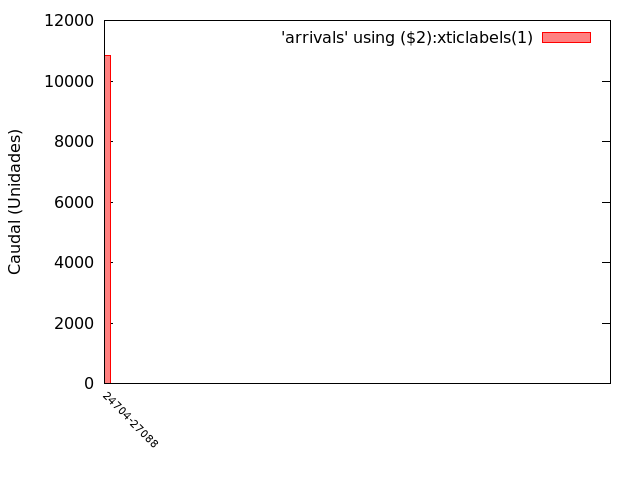
\includegraphics[width=0.8\textwidth]{imgs/mem_times.png}
	\end{center}

	\emph{Importante:} este script solo funciona si no se han indicado 2 puertos como parámetros.

	\item \textbf{hist\_sizes.png} Genera un histograma (en imgs/sizes.png) con cuantos paquetes ha habido de cada tamaño 
	\begin{center}
	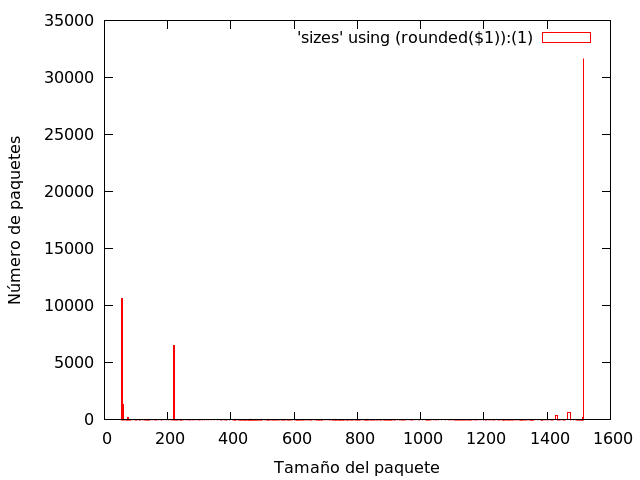
\includegraphics[width=0.8\textwidth]{imgs/mem_sizes.png}
	\end{center}
	\item \textbf{hist\_port.png} Genera un histograma (en imgs/arrivals\_port.png) a partir del fichero arrivals (que contiene los tiempos de llegadas de cada paquete entre los 2 puertos especificados). El ancho del histograma es de 0.05 segundos.

	Para generar este ejemplo se han utilizado los puertos 
	\begin{itemize}
		\item origen: 80
		\item destino:55865
	\end{itemize}
	y descartado los pocos paquetes que han tardado más de 1.5 segundos en llegar para ejemplificar mejor el histograma generado por este fichero.
	\begin{center}
	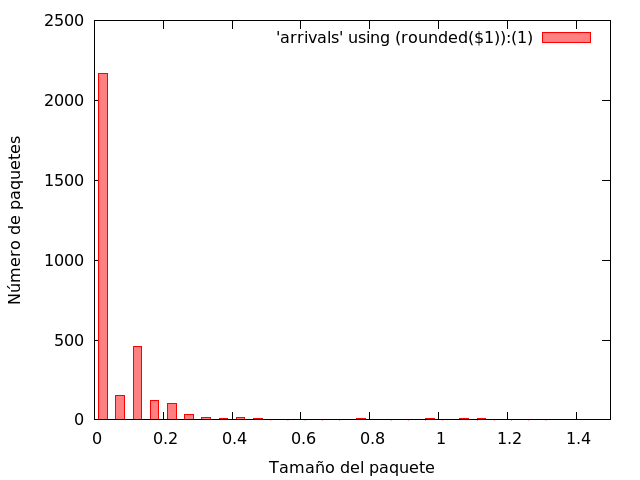
\includegraphics[width=0.8\textwidth]{imgs/mem_arrivals_port.png}
	\end{center}
\end{itemize}


\end{document}